%!TEX root = ../thesis.tex

\newpage
    \section*{Мета роботи:}
    \qquad  Ознайомлення з принципами баєсiвського пiдходу в криптоаналiзi, побудова детермiнiстичної та стохастичної вирiшуючих функцiй для моделей схем шифрування та криптоаналiз моделей шифрiв за допомогою програмної реалiзацiї, зокрема здiйснення порiвняльного аналiзу вирiшуючих функцiй.

    \section*{Завдання}

    \begin{enumerate}
    \item  Ознайомитись з порядком виконання комп’ютерного практикуму та вiдповiдними вимогами до виконання роботи.
    \item Уважно прочитати необхiднi теоретичнi вiдомостi до комп’ютерного практикуму.
    \item Для заданого варiанта моделi шифру описати алгоритм побудови детермiнiстичної та стохастичної вирiшуючих функцiй. Створити репозиторiй в системi контролю версiй Git (бажано використовувати вебсервiс GitHub). Важливо:
    
    (а) репозиторiй створюється перед початком роботи над програмним кодом (якщо репозиторiй приватний, то перед початком роботи має бути надано доступ викладачу до даного репози- торiю);
        
    (б) весь процес створення програмного коду має бути вiдображений у вiдповiдних комiтах про- екту (для кожної атомарної змiни коду має бути власний комiт);
        
    (в) програмна реалiзацiя не допускається до захисту при недотриманнi вищевизначених вимог.
        
    \item Реалiзувати алгоритми програмно i подати результати побудови детермiнiстичної та стохастичної вирiшуючих функцiй у виглядi таблиць. Для цього необхiдно:
    
    (а) порахувати розподiли $P(C)$ та $P(M,C)$;
    
    (б) ґрунтуючись на цих розподiлах обчислити $P(M|C)$;
    
    (в) побудова оптимальних детермiнiстичної та стохастичної вирiшуючих функцiй зводиться до максимiзацiї $P(M|C)$.
    
    \item Обчислити середнi втрати, провести порiвняльний аналiз вирiшуючих функцiй.
    \end{enumerate}
    \begin{bf}
    Варіант завдання:
    \end{bf}
    16\\
\newpage
    \begin{center}
        \begin{Large}
            Хід роботи
        \end{Large}
    \end{center}
    
\section*{Опис алгоритму побудови детермiнiстичної та стохастичної вирiшуючих функцiй}
    
Для побудови детерміністичної функції використовувались значення $P(M|C)$ так, що $ \delta_{d}(C)  = index ~ \displaystyle\max_{M} P(M|C)$.
\\

Стохастична функція зберігає усі максимуми, тому вона будувалась так що в кожному рядку матриці на місцях максимальних елементів вона дорівнювала $(1 ~~ / $ кількість максмимальних елементів у рядку$)$, а на місцях не максимальних елементів дорівнювала нулю.
    
\newpage

\textbf{Таблиця $P(M|C)$ для 16 варіанту }
\begin{figure}[h!]
\center{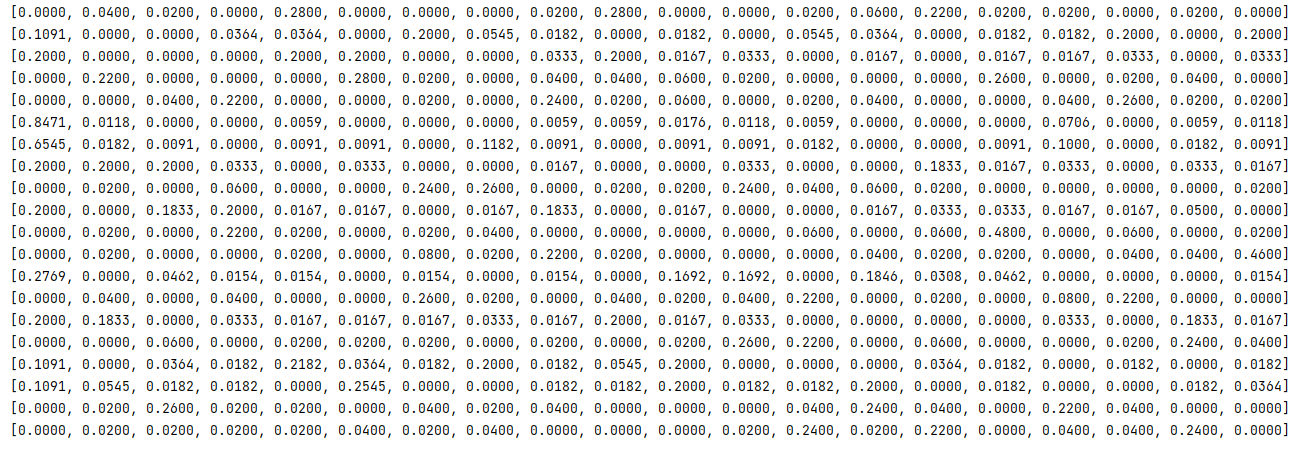
\includegraphics[scale=0.5]{1.png}}
\label{fig:image}
\end{figure}
    
\textbf{Таблиця $P(M|C)$ для 6 варіанту } 
\begin{figure}[h!]
\center{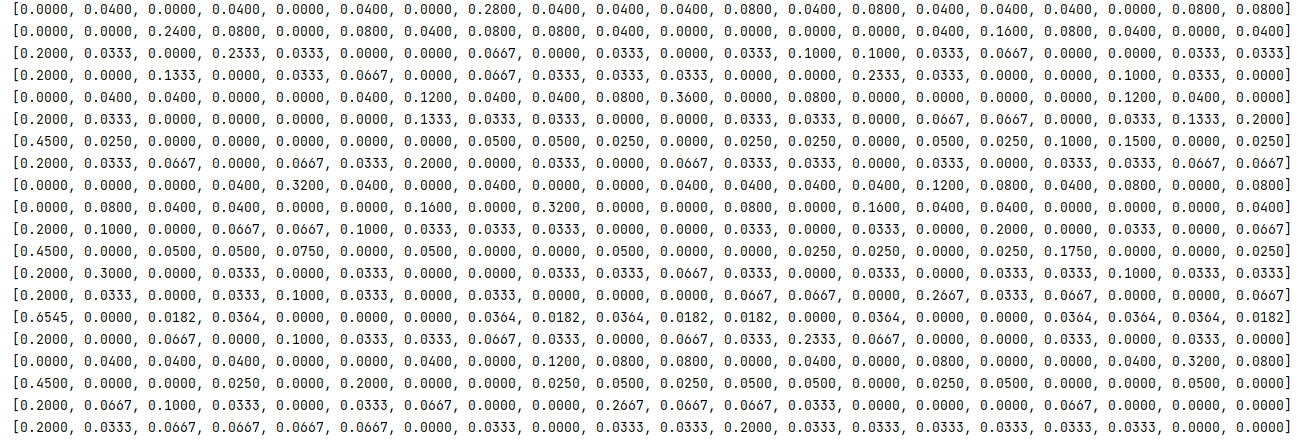
\includegraphics[scale=0.5]{2.png}}
\label{fig:image}
\end{figure}  
 
\newpage

\textbf{Знайденi детермiнiстична та стохастична функцiї у виглядi таблиць для 16 варіанту}
\\

Детерміністична функція:\\
\begin{figure}[h!]
\center{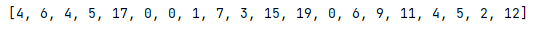
\includegraphics[scale=0.5]{3.png}}
\label{fig:image}
\end{figure}  
    
Стохастична функція:\\
\begin{figure}[h!]
\center{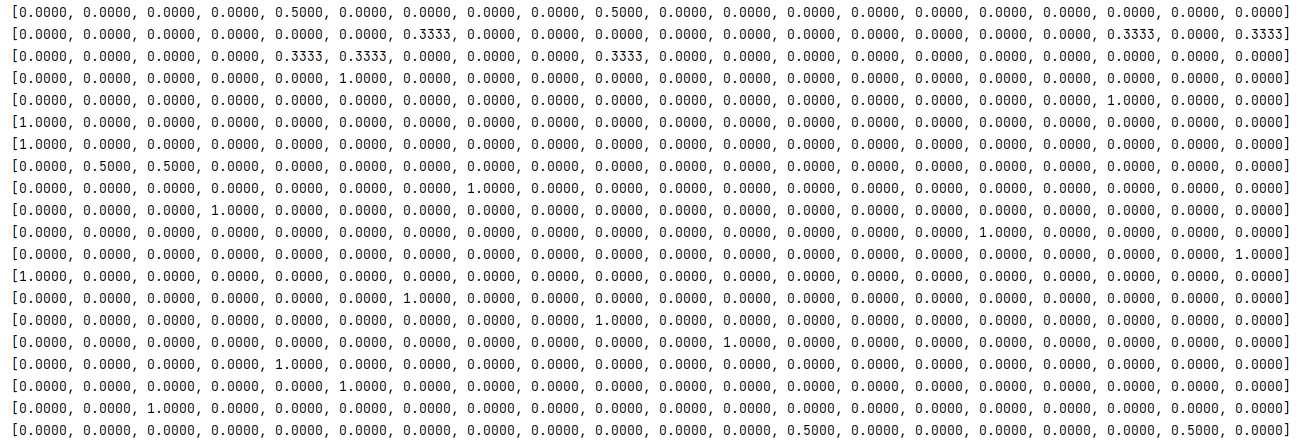
\includegraphics[scale=0.5]{4.png}}
\label{fig:image}
\end{figure}    

\newpage
\textbf{Знайденi детермiнiстична та стохастична функцiї у виглядi таблиць для 6 варіанту}
\\

Детерміністична функція:\\
\begin{figure}[h!]
\center{
\includegraphics[scale=0.5]{6.png}}
\label{fig:image}
\end{figure}      

Стохастична функція:\\
\begin{figure}[h!]
\center{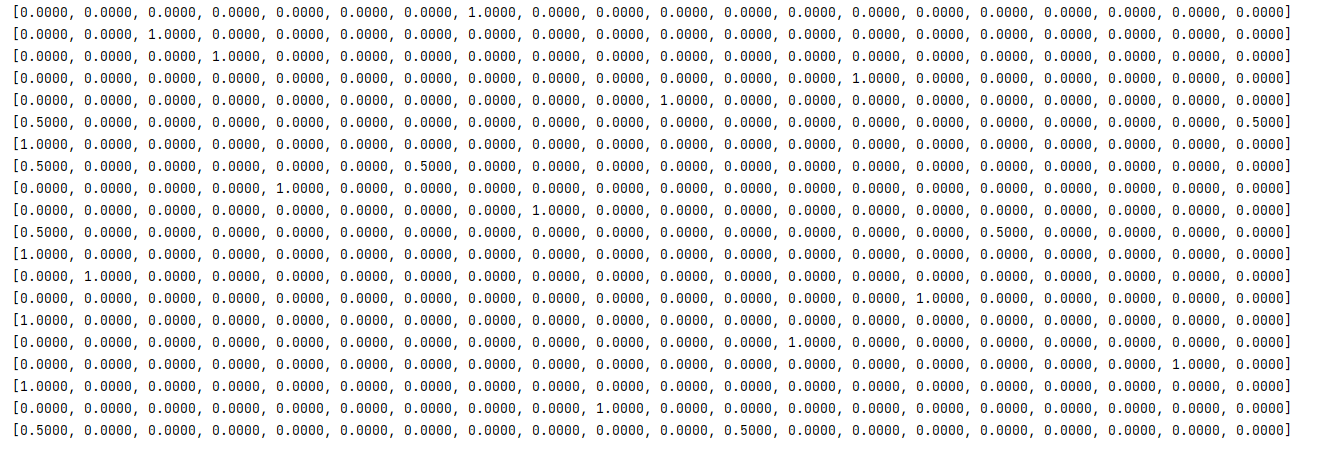
\includegraphics[scale=0.5]{5.png}}
\label{fig:image}
\end{figure}      


\newpage
\textbf{Cереднi втрати для вирiшуючих функцiй для 16 варіанту}
\\

Для детерміністичної вирішуючої функції : \textbf{0.6232000000000001}
\\

Для стохастичної вирішуючої функції : \textbf{0.6232000000000001} 
\\
    
\textbf{Cереднi втрати для вирiшуючих функцiй для 6 варіанту}
\\
   
Для детерміністичної вирішуючої функції: \textbf{0.6703999999999998} 
\\

Для стохастичної вирішуючої функції: \textbf{0.6703999999999998} 
\\


\textbf{Опис труднощiв, що виникали при виконаннi комп’ютерного практикуму, та шляхи їх розв’язання:}
\\

Під час виконання лабораторної роботи виникли невеликі труднощі з побудовою ймовірностей та розумінням, як саме необхідно будувати стохастичну вирішуючу функцію, а також була проблема в похибці при операціях з числами з плаваючою точкою.
\\  

\textbf{Порівняльний аналіз детерміністичної і стохастичної вирішуючих функцій}
\\

При виконанні даної роботи було побудовано детерміністичну і стохастичку вирішувані функції, а також було пораховано середні втрати для детермінстичної і стохастичної вирішуваних функцій. Після виконання роботи був проведений аналіз роботи цих функцій і був зроблений висновок, що обидві функції є однаково ефективними, оскільки середні втрати для обох функцій однакові.